% Copyright 2023 Kieran W Harvie. All rights reserved.

\section{Quick Summary of Spaces}
A space is a collection of elements, often called points,
with some additional structure.
There are four main types of spaces that form a nice hierarchy,
that is that some types of spaces are always a subtype of other space.
\subsection{Hierarchy}
{\textbf{Topological Space: Neighbourhood}}
In a topological space the elements have a concept of "Neighbourhood",
that is the points which are adjacent to each point.
\begin{center}
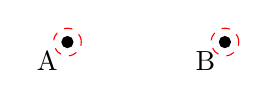
\begin{tikzpicture}
	\draw[dashed,red] (0,0) circle (5pt); 
	\filldraw (0,0) node[below left] {A} circle (2pt);
	\draw[dashed,red] (2,0) circle (5pt); 
	\filldraw (2,0) node[below left] {B} circle (2pt);
\end{tikzpicture}
\end{center}

{\textbf{Metric Space: Distance}}
In a metric space the element have a concept of distance to each other.
You can induce a neighbourhood by saying all points within a certain threshold distance to a point are in the neighbourhood of that point.
\begin{center}
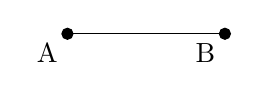
\begin{tikzpicture}
	\draw (0,0) -- (2,0);
	\filldraw (0,0) node[below left] {A} circle (2pt);
	\filldraw (2,0) node[below left] {B} circle (2pt);
\end{tikzpicture}
\end{center}

{\textbf{Normed Space: Length}}
In a normed space there is a concept of length of a point.
Shown here as their distance to some origin.
A distance can be induced by getting the length of an arrow going from A to B.
\begin{center}
\begin{tikzpicture}
	\draw[->] (0,0) -- (0,3.8);
	\draw[->] (0,0) -- (1.9,2.9);
	\filldraw (0,0) node[below] {O} circle (2pt);
	\filldraw (0,4) node[left] {A} circle (2pt);
	\filldraw (2,3) node[right] {B} circle (2pt);
\end{tikzpicture}
\end{center}


{\textbf{Inner-product Space: Projection}}
An inner product space has a concept of projecting one element on another.
You can induce a length by projecting an object onto itself.
\begin{center}
\begin{tikzpicture}
	\draw[->] (0,0) --(0,4.8);
	\draw[->] (0,0) -- (1.9,1.9);
	\draw[red,dashed] (2,2) -- (0,4);
	\draw (1.7,2.3) -- (1.4,2) -- (1.7,1.7);
	\filldraw (0,0) node[below] {O} circle (2pt);
	\filldraw (0,5) node[left] {A} circle (2pt);
	\filldraw (2,2) node[right] {B} circle (2pt);
	\filldraw (0,4) node[left] {B$'$} circle (2pt);
\end{tikzpicture}
\end{center}

\subsection{Euclidean}
Euclidean space is a normed space on $\mathbb{R}^n$ where the inner product is given by $\sum_k A_kB_k$.
This naturally induces a metric on $\mathbb{R}^n$.

The reason we care about the metric of Euclidean space is because all normed spaces have a form of the Pythagorean theorem.
Making metric space the most endowed space we can easily start thinking about non-Euclidean space.

This sucks because most talk about non-Euclidean space talks about "parallel lines" which makes one naturally think about angles and hence an inner product.
But no, instead we have the concept of a geodesic.
A geodesic is a curve that is locally distance minimizing.
This locality comes from the topology, and means that for all points $\gamma(t_1)$ and $\gamma(t_0)$ on the curve $\gamma$ such that they are in the same neighbourhood satisfy:
\[ d(\gamma(t_1),\gamma(t_0)) = k|t_1-t_2|\]

\subsection{non-Euclidean}
Quick rundown of some attempts of non-Euclidean geometries:

Pseudo-Euclidean: Like how we defined Euclidean Space was defined with an inner product we define a new structure with a different quadratic form.
\\

Riemann Manifold: A Manifold is a space that is "locally Euclidean". And a Riemann Manifold is one where this inner-product in the local Euclidean space is always positive.\\

Pseudo-Riemann Manifold: Like A Riemann Manifold but the inner-product is only required to be non-degenerate. I think this includes Pseudo-Euclidean space, but haven't put much thought into it.
